\pdfoutput=1
\documentclass[pra,twocolumn,showpacs,amsmath,amssymb]{revtex4-2}

\usepackage{graphicx}%Include figure files
\usepackage{dcolumn}%Align table columns on decimal point
\usepackage{bm}% bold math
\usepackage[section]{placeins} %force no floats before section
\usepackage{float}

\setlength{\parskip}{1em}

%\nofiles

\begin{document}

\title{Project 4: First and Second Order Phase Transitions in the Ising
Model of Ferromagnetism}


\author{Christopher McGlinn}
\affiliation{Department of Physics and Astronomy, University
of Delaware, Newark, DE 19716-2570, USA}

\begin{abstract}
We explore how temperature and external fields effect a series of spins in an Ising model. For this we will use the Metropolis Monte Carlo algorithm for a two-dimensional lattice system. This system will be subjected to different temperatures and external fields. The goal is to show the phase transitions of the different systems and how temperature and external fields play a part in that.
\end{abstract}

\pacs{63.70.+h}


\maketitle

\section{Introduction} \label{sec:intro}

In 1920, Wilhelm Lenz developed a model for representing ferromagnetism in statistical mechanics. This model was given to Ernst Ising who solved it for a one-dimensional lattice in 1924. The two-dimensional system would later be solved by Lars Onsager in 1944. In this model, the system is represented by a lattice. The spins of the different elements are represented by a -1 and a 1 and are allowed to interact with their neighbors. An algorithm to solve this system would be developed know as the Metropolis Monte Carlo algorithm, which is the algorithm we will use to understand this system.
\par In the algorithm, the energy of the system is represented by the following equation:
\begin{eqnarray}
E = -J\sum_{<i,j>}S_i S_j - H\sum_i S_i
\end{eqnarray}
\par Here, J is the exchange coupling and H is the external field. The exchange coupling is multiplied by the sums of the neighboring spins and the external field is multiplied by the spin itself.
\par In the algorithm, we go through the entire lattice. For each item, we flip the spin and see if the energy is lower. If it is, we keep that spin. If it is not, we compare it to a random number between 0 and 1 and see if it is lower than that and keep the spin if it does.
\par Furthermore, we will evaluate certain thermodynamic quantities across different system. The first quantity will be the mean magnetization represented by the following equation:
\begin{eqnarray}
<\bar{M}> = \frac{1}{N_{MC}}\sum_{\alpa=1}^{N_{MC}}\bar{M_\alpha}
\end{eqnarray}
Another important quantities are the specific heat per spin and the susceptibility per spin represented, respectively, by the following equations:
\begin{eqnarray}
C_V = \frac{1}{N_{s}}\frac{1}{k_B T} (<E>^2 - <E^2>) \\
\chi = \frac{1}{N_{s}}\frac{1}{k_B T} (<M>^2 - <M^2>) \\
\end{eqnarray}
\par With these quantities, we will successfully evaluate the system.

\section{Method} \label{sec:method}

First we must define the set of variables for the system. To begin we will introduce a set of dimensionless variables to govern the interactions in the system. :
\begin{align}
\bar{E} &= \frac{E}{E_o} \notag \\
\bar{T} &= \frac{T}{T_o} \notag
\end{align}
To evaluate this further, we will need to look at the probability of a particular system of spins:
\begin{align}
    P_\alpha = \frac{e^{-\frac{E_\alpha}{k_b T}}}{Z}
\end{align}
We can then relate this to the average energy:
\begin{align}
<E> = \sum E_\alpha P_\alpha = \frac{1}{Z} \sum_\alpha E_\alpha e^{-\frac{E_\alpha}{k_b T}} \notag
\end{align}
Thus, we can define the normalization constants as such:
\begin{align}
E_o = J \notag \\
T_o = \frac{E_o}{k_B} \notag
\end{align}
This gives us the following result:
\begin{align}
    <E> = \frac{1}{Z} \sum E_\alpha e^{-\frac{\bar{E}}{\bar{T}}}
\end{align}
These equations will allow us to explore the system with only a dependence on H and T. For this system, the critical temperature occurs at $T = 2.269$ and the number of metropolitan steps run for each system was 1000.

\section{Results} \label{sec:results}

To begin, we will look at the systems at equilibrium for different temperatures.
\par In figure 1, we see the systems at equilibrium for different values of T. We can see that the systems are the same across the different temperatures. Thus the temperature has no effect on the equilibrium state.
\par However, when we look at figure 2, we also see that the external field plays a minor role in the final state.
\par First, we will evaluate the system as the external field increases and then decreases back to its original value. We set all the spins of a 128x128 lattice to -1 and run the algorithm until it reaches equilibrium for each value of H. We can see this in figure 3.
\par For the value of $T = 1$, as the external field increases, the average magnetization remains the same until around where the external field no longer exists. Then there is a phase transition where all of the spins reach a value of 1. As the external field decreases back down to its original value, it also experiences a phase transition, however, at a different value of H. The system waits until there is a sufficient opposing magnetic field to then start flipping the spins.

\begin{figure}[t!]
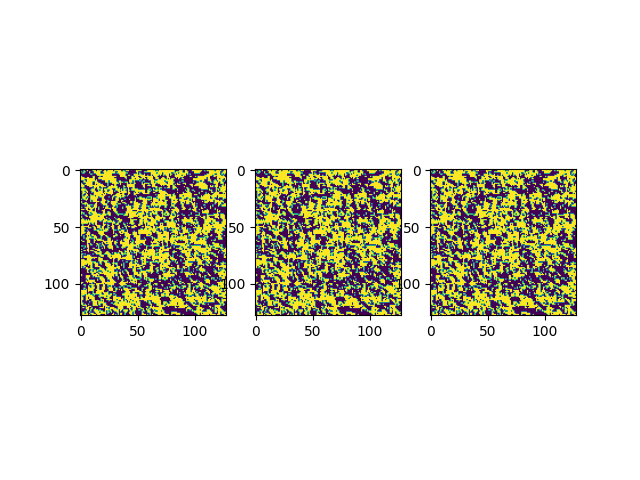
\includegraphics[scale=0.5]{Lattice.png}
\caption{128x128 Lattice after 1000 metropolitan steps for $T = 1, 2.269, 4$}\label{Poincare0.5}
\end{figure}

\begin{figure}[t!]
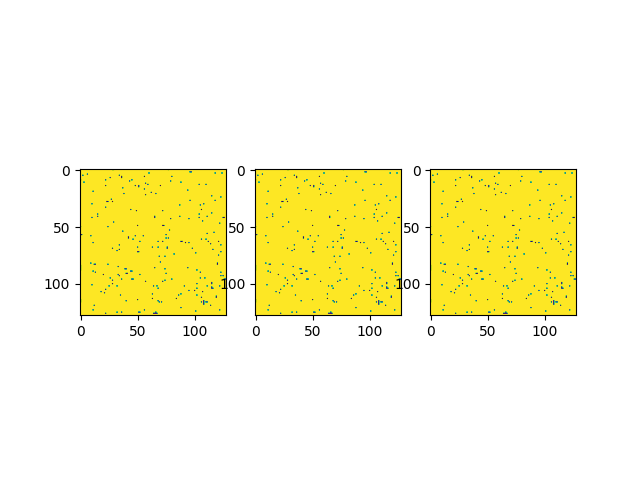
\includegraphics[scale=0.5]{LatticeH.png}
\caption{128x128 Lattice after 1000 metropolitan steps for $H = -2.5, 0, 2.5$}\label{Poincare0.5}
\end{figure}

\begin{figure}[t!]
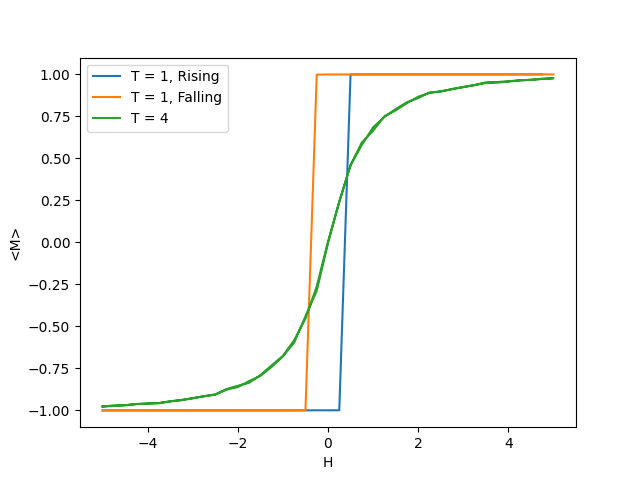
\includegraphics[scale=0.50]{Figure_1.png}
\caption{Average magnetization of for given external field values.}\label{Poincare1}
\end{figure}

\par This phase transition, while continuous, is only first order. However, since the temperature is below the critical temperature of the system, spin flipping is much less likely to occur.
\par This is further explained when looking at a system that is where flipping is more likely to occur. In figure 3, the transition of the magnetization from -1 to 1 is a more smooth transition. The figure displays a second order transition. Since there is more energy in the system, spin flipping is more likely to occur. This allows for them to occur at values closer to 0, ever when the field is opposing the spin.

\begin{figure}[t!]
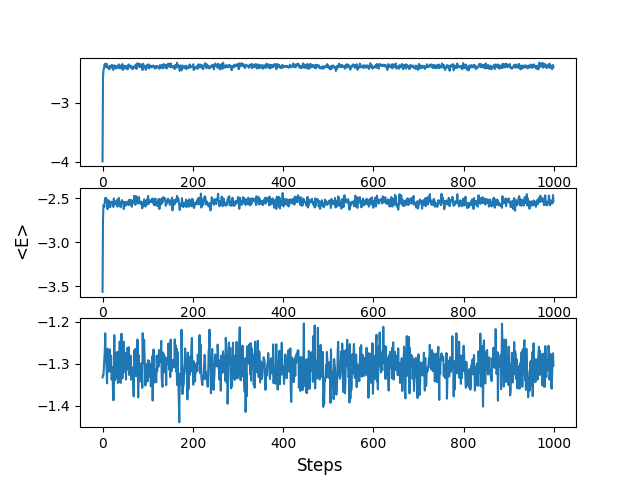
\includegraphics[scale=0.50]{e_steps.png}
\caption{Energy compared to the number of metropolitan steps for $T = 1, 2.269, 4$}\label{Poincare9}
\end{figure}

\begin{figure}[t!]
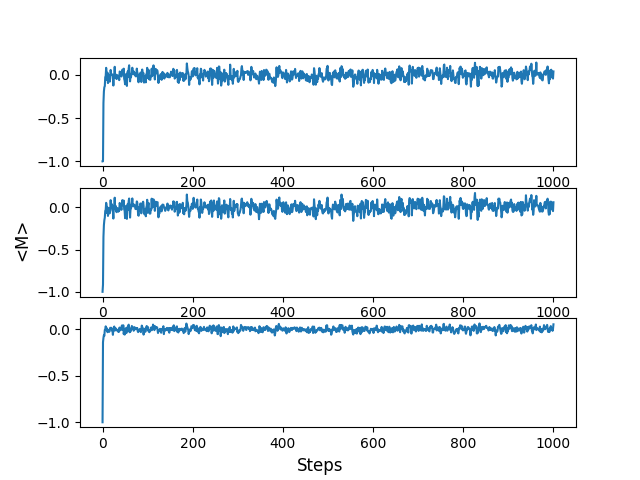
\includegraphics[scale=0.50]{m_steps.png}
\caption{Magnetization compared to the number of metropolitan steps for $T = 1, 2.269, 4$}\label{autocorr}
\end{figure}

\par It is also important to look at how many steps a system needs to reach equilibrium. For this, we compared the magnetization and energy to the number of steps in the system. In figures 4 and 5, we see that as the temperature rises, a steadier equilibrium is achieved at a lower steps value. When the temperature is below the critical temperature, equilibrium is achieved at a much later time then when the temperature is above the critical temperature.
\par From this, we can determine that the system, in the absence of an external field, will require more steps to reach equilibrium for lower values of T. This will be further amplified by introducing an external field to the system. An external field would cause the system to require more steps to reach equilibrium.

\begin{figure}[t!]
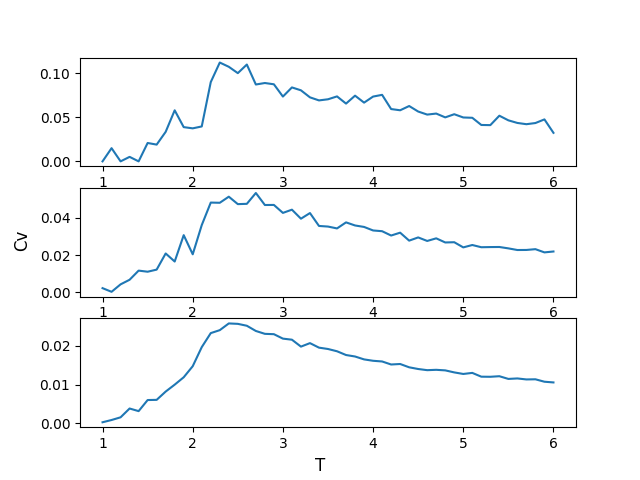
\includegraphics[scale=0.50]{cv_t.png}
\caption{Heat capacity compared to temperature for lattices of size 16x16, 32x32, and 64x64}\label{Poincare0.5}
\end{figure}

Finally we can look at the heat capacity as it changes over a range of temperatures. In figure 6, we can see this change. We see that the heat capacity increases until the temperature reaches the critical temperature. At greater temperatures, the heat capacity decreases. In a smaller lattice, the heat capacity has a greater amplitude than that of the larger lattices. This is likely due to the number of interactions in the system.
\par It is also worth pointing out the fluctuations in the graph. At smaller lattices, there is a much more likely chance for the system to spontaneously flip. As we can see with the larger lattice size, this is much less likely to happen and the graph is smoother.

\section{Conclusion} \label{sec:conclusion}

In conclusion, we were able to successfully display how the Ising model changes with different parameters. In temperatures below the critical temperature, the transition between spins is a first order transition, but above it it is second order. As the temperature rises in the system, there are more spontaneous spin flips and thus the system is more likely to reach its equilibrium at lower steps. It also points out that a larger lattice size is needed to leave out inconsistencies. 

\begin{thebibliography}{9}
\bibitem{}Nicholas J. Giordano and Hisao Nakanish, \emph{Computational Physics}, (Pearson Prentice Hall, Upper Saddle River NJ,2006).
\end{thebibliography}

\end{document}